\documentclass[hyperref=colorlinks]{beamer}
\mode<presentation>
\usetheme{iclpt}
\setbeamertemplate{navigation symbols}{}
\setbeamertemplate{headline}{
\begin{beamercolorbox}[leftskip=.2cm,rightskip=.2cm,topskip=.2cm,ht=1.1cm,dp=0.1cm,wd=\textwidth]{institute in head/foot}
  
\includegraphics[height=1cm]{icl.pdf}
  \hfill
  
\includegraphics[height=1cm]{../Pics/CMS-Color.pdf}
\end{beamercolorbox}
}
\setbeamertemplate{footline}{
\begin{beamercolorbox}[ht=.55cm,dp=0.4cm,wd=\textwidth,leftskip=.3cm]{author in head/foot}%
  \begin{minipage}[c]{5cm}%
    \usebeamerfont{author in head/foot}
    \insertshortauthor 
    \insertshorttitle
    \end{minipage}\hfill%
  \insertframenumber{} / \pageref{lastframe}
  \hfill
  \begin{minipage}{6cm}
    \hfill
  \end{minipage}
\end{beamercolorbox}%
}

\usepackage{color}
\usepackage{tabularx,colortbl}
\usepackage{graphicx}
\usepackage{pdfpages}
\usepackage{feynmp}
\usepackage{tikz}
\usetikzlibrary{calc, shapes, backgrounds,arrows,positioning}
\DeclareGraphicsRule{*}{mps}{*}{}

\title{\vspace{-0.2cm} VBF Higgs to Invisible}
\subtitle{\vspace{-0.7cm}}
\author[]{}%\underline{P. Dunne}} % A.M. Magnan and A. Nikitenko Joao Pela with \\ R. Aggleton, J. Brooke: Bristol \\ C.Asawangtrakuldee, Q.Li: Peking \\ P. Srimanobhas: Chulalongkorn \\ S. Kumar, K. Mazumdar: Mumbai}
\titlegraphic{
  \vspace{-0.7cm}
  %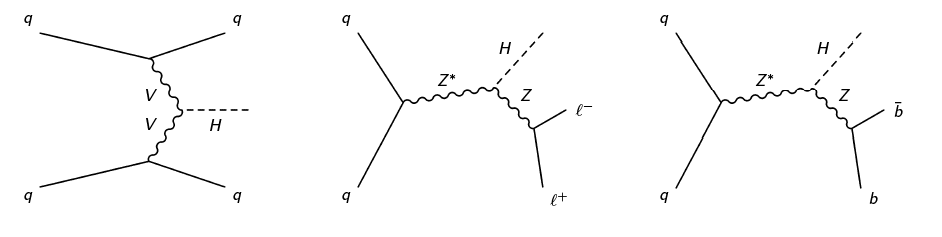
\includegraphics[width=\textwidth]{TalkPics/invcomb021213/feyndiags}
  %% \begin{fmfgraph*}(100,70)
  %%         \fmfleft{i1,i2}
  %%         \fmfright{o1,o2,o3}
  %%         \fmf{fermion}{i1,v1,o1}
  %%         \fmf{fermion}{i2,v2,o3}
  %%         \fmf{phantom,tension=4/5}{v1,v2}
  %%         \fmffreeze
  %%         \fmf{photon,label=$W,,Z$}{v1,v3}
  %%         \fmf{photon,label=$W,,Z$}{v2,v3}
  %%         \fmf{dashes}{v3,o2}
  %%         \fmflabel{$q$}{i1}
  %%         \fmflabel{$q$}{i2}
  %%         \fmflabel{$q$}{o1}
  %%         \fmflabel{$q$}{o3}
  %%         \fmflabel{$H$}{o2}
  %%       \end{fmfgraph*}
}
\date{}
\begin{document}
\begin{fmffile}{higgsexoupdatefeyndiags}
\tikzstyle{every picture}+=[remember picture]

%TITLE PAGE
\section{Title}
\begin{frame}
  \titlepage
  
\end{frame}

\begin{frame}
  \frametitle{Reminder}
  \begin{block}{}
    \begin{itemize}
    \item Signal samples shown previously had some reco selection applied
    \item Light trees now made with no skimming applied
    \item Gen level information will be shown
    \end{itemize}
    \end{block}
\end{frame}

\begin{frame}
  \frametitle{Signal Comparison: run 1 vs run 2: Gen Jet $p_{T}$}
  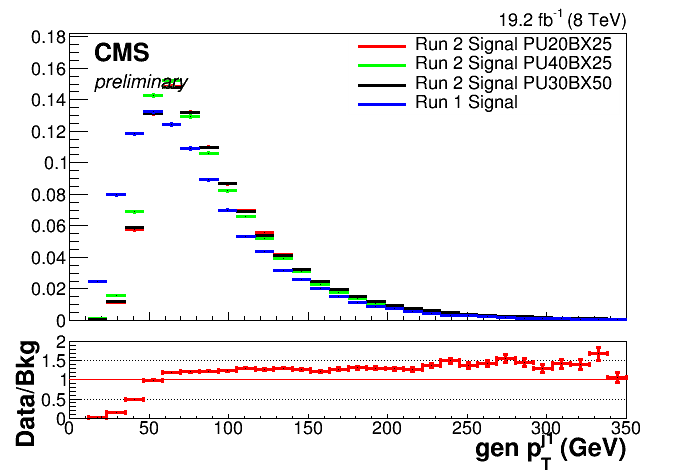
\includegraphics[width=.5\textwidth]{TalkPics/unskimmedsigmc060715/output_run1comparegen060715/nunu_norm_genjet1_pt}
  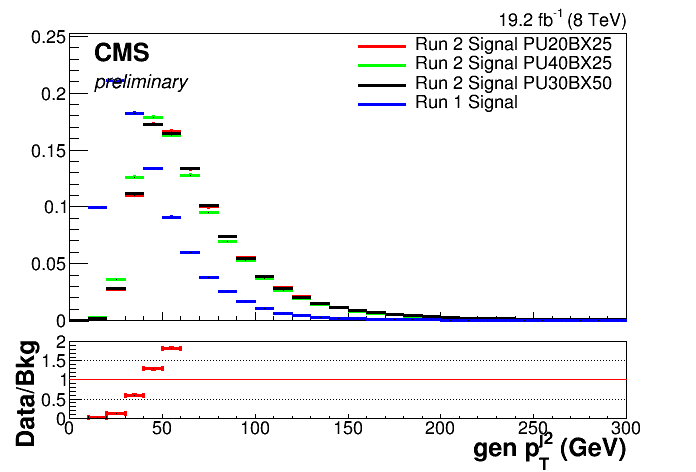
\includegraphics[width=.5\textwidth]{TalkPics/unskimmedsigmc060715/output_run1comparegen060715/nunu_norm_genjet2_pt}
  \begin{block}{}
    \begin{itemize}
    \item More as expected, higher pt in run 2
    \end{itemize}
  \end{block}
\end{frame}

\begin{frame}
  \frametitle{Signal Comparison: run 1 vs run 2: Gen Jet $\eta$}
  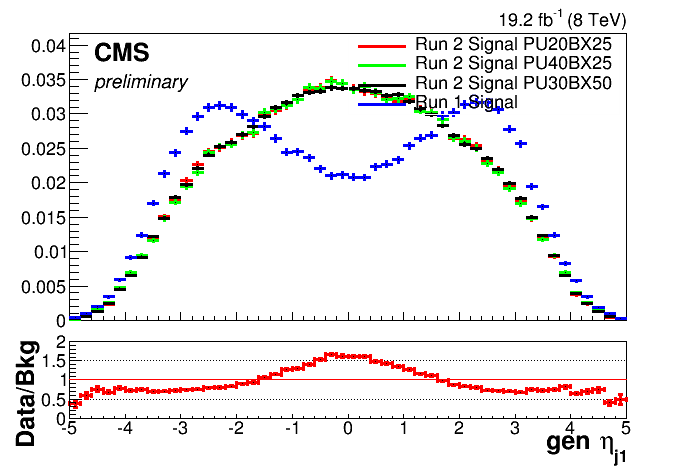
\includegraphics[width=.5\textwidth]{TalkPics/unskimmedsigmc060715/output_run1comparegen060715/nunu_norm_genjet1_eta}
  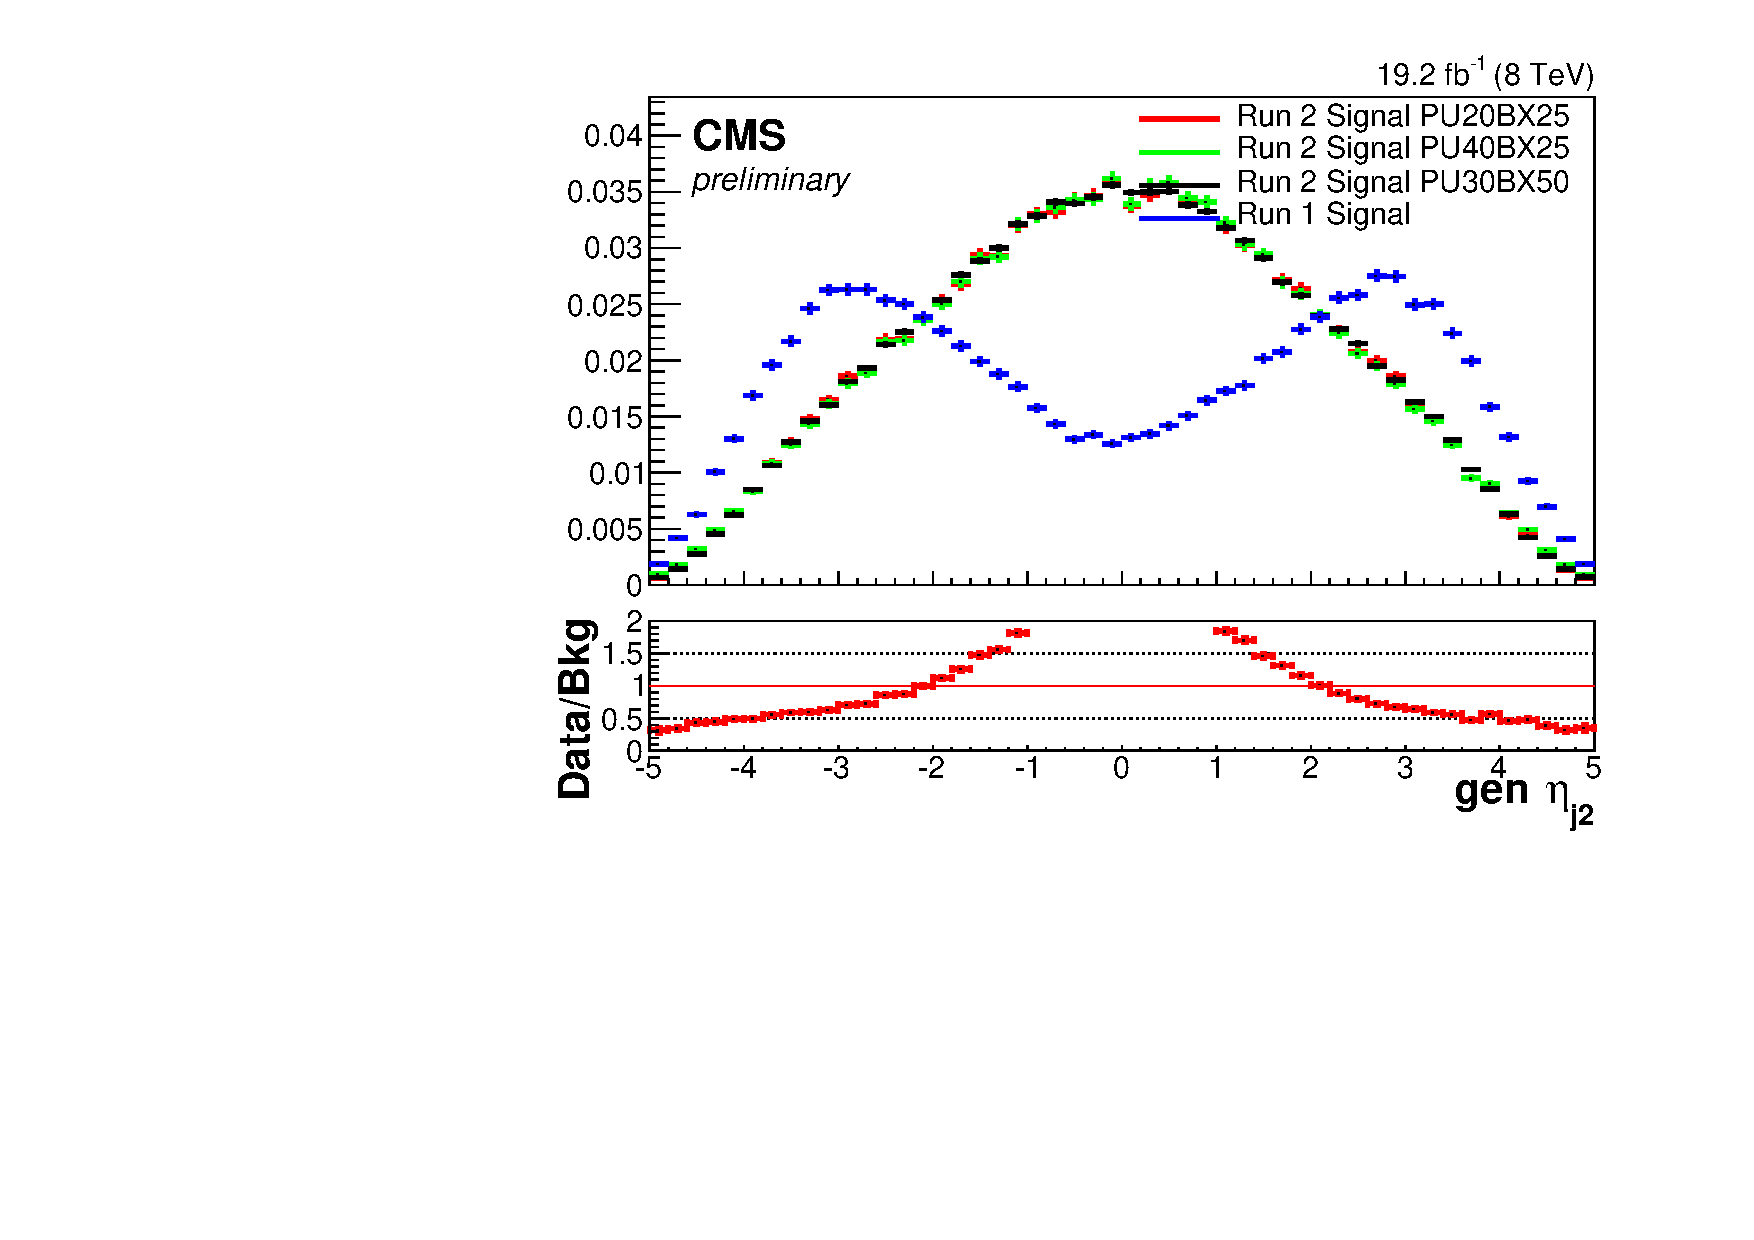
\includegraphics[width=.5\textwidth]{TalkPics/unskimmedsigmc060715/output_run1comparegen060715/nunu_norm_genjet2_eta}
  \begin{block}{}
    \begin{itemize}
    \item Run 2 jets seem to have much lower $\eta$
    \end{itemize}
  \end{block}
\end{frame}

\begin{frame}
  \frametitle{Signal Comparison: run 1 vs run 2: Gen Jet $\phi$}
  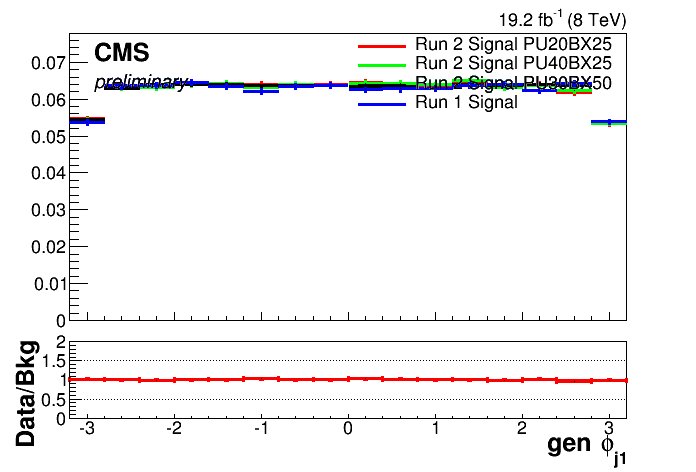
\includegraphics[width=.5\textwidth]{TalkPics/unskimmedsigmc060715/output_run1comparegen060715/nunu_norm_genjet1_phi}
  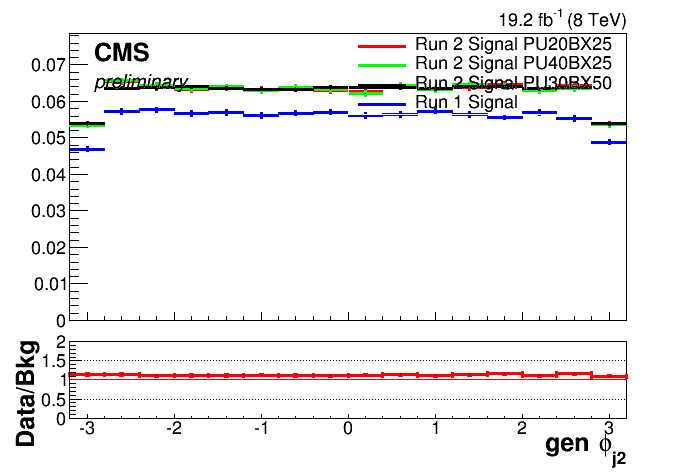
\includegraphics[width=.5\textwidth]{TalkPics/unskimmedsigmc060715/output_run1comparegen060715/nunu_norm_genjet2_phi}
  \begin{block}{}
    \begin{itemize}
    \item $\phi$ is flat as expected
    \end{itemize}
  \end{block}
\end{frame}

\begin{frame}
  \frametitle{Signal Comparison: run 1 vs run 2: Gen Jet angle differences}
  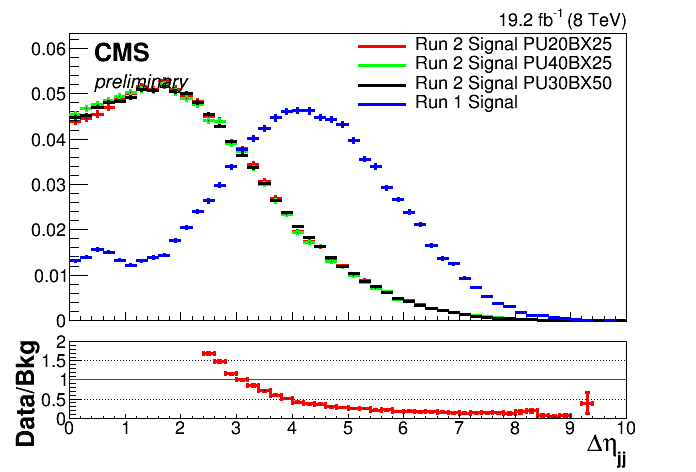
\includegraphics[width=.5\textwidth]{TalkPics/unskimmedsigmc060715/output_run1comparegen060715/nunu_norm_digenjet_deta}
  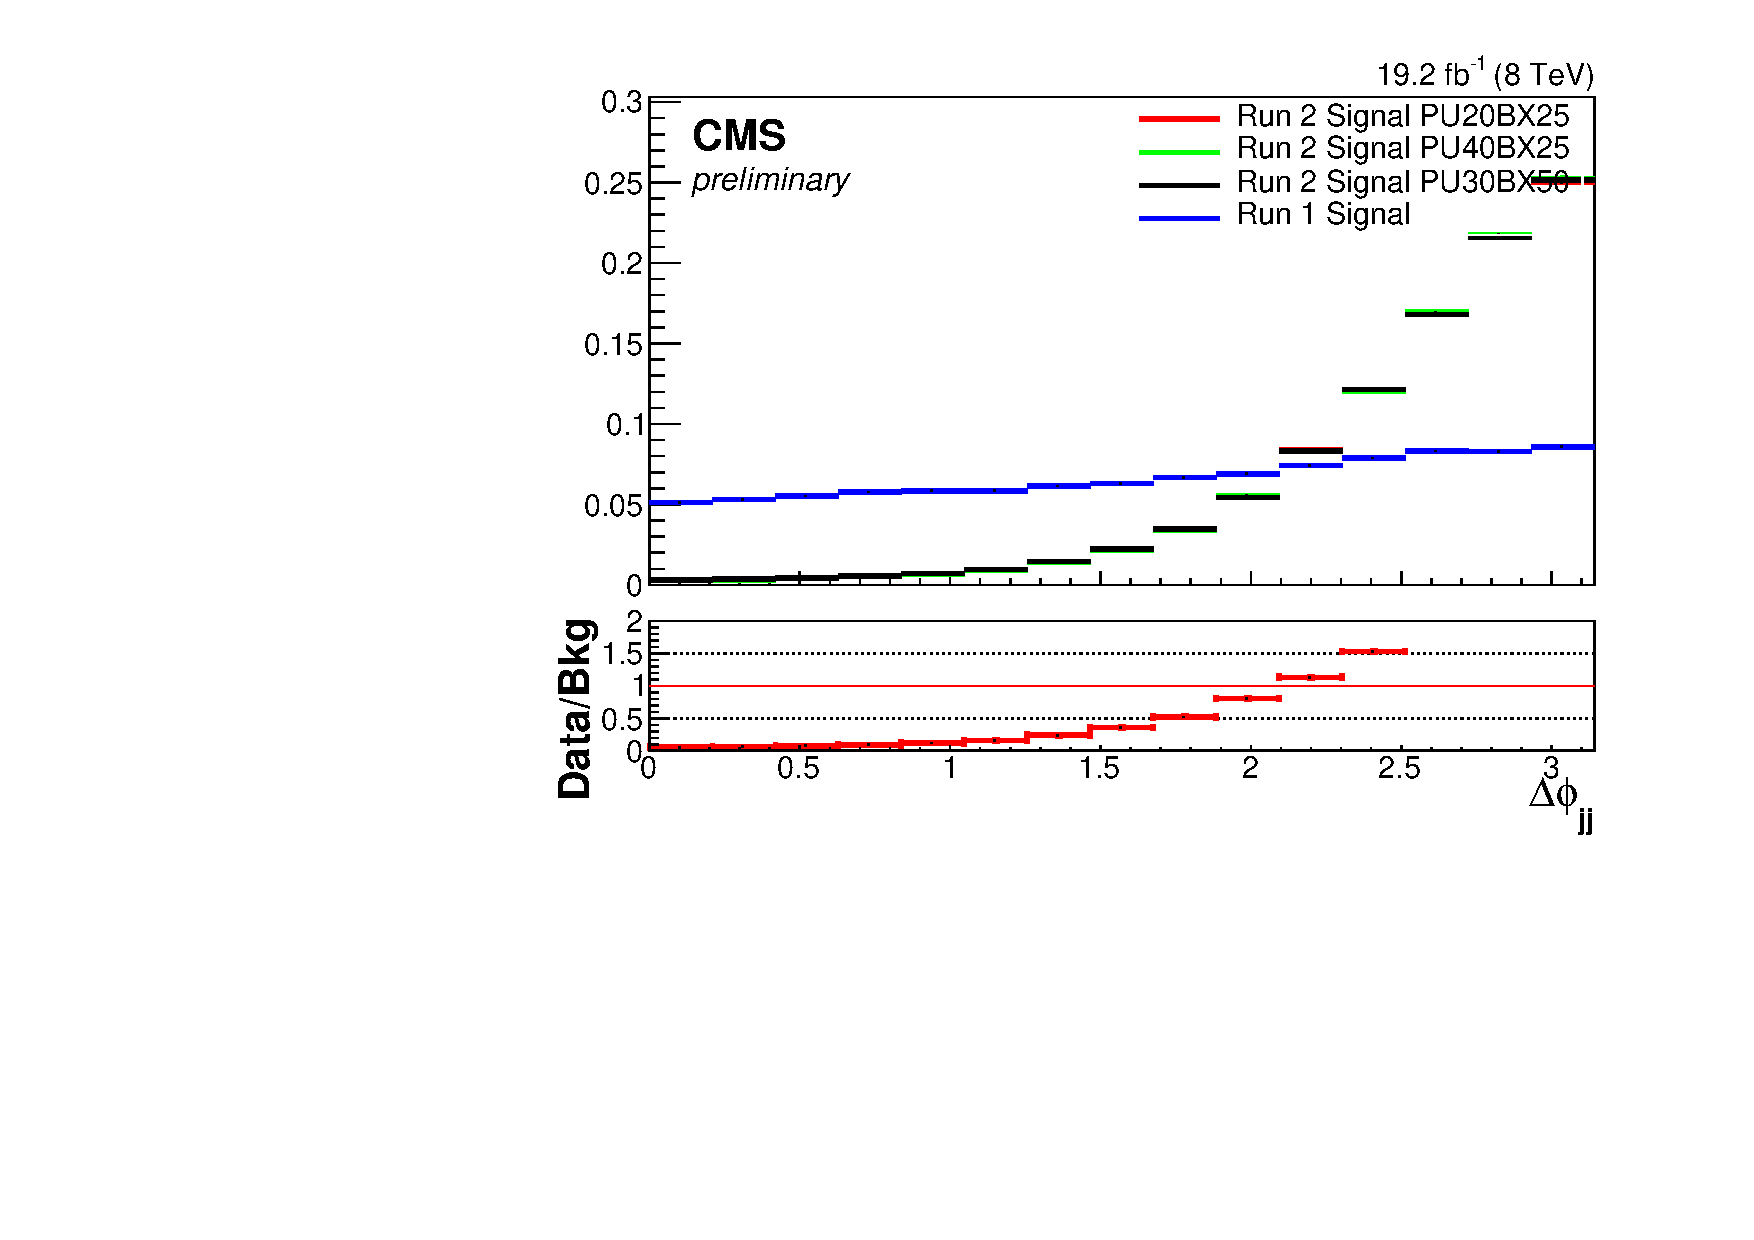
\includegraphics[width=.5\textwidth]{TalkPics/unskimmedsigmc060715/output_run1comparegen060715/nunu_norm_digenjet_dphi}
  \begin{block}{}
    \begin{itemize}
    \item Run 2 jet angle differences are completely different
    \end{itemize}
  \end{block}
\end{frame}

\begin{frame}
  \frametitle{Signal Comparison: run 1 vs run 2: Gen Jet Mass}
  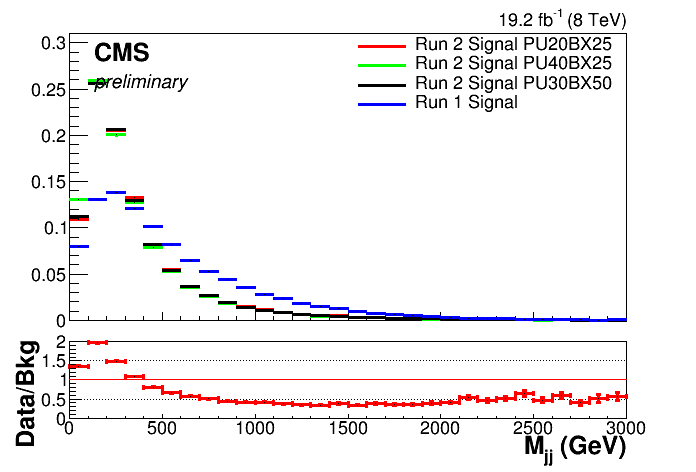
\includegraphics[width=.5\textwidth]{TalkPics/unskimmedsigmc060715/output_run1comparegen060715/nunu_norm_digenjet_M}
  \begin{block}{}
    \begin{itemize}
    \item $M_{jj}$ also very different, probably due to different angle distributions
    \end{itemize}
  \end{block}
\end{frame}

\begin{frame}
  \frametitle{Gen jet differences}
  \begin{block}{}
    \begin{itemize}
    \item Looked through all gen jets and reco jets in the event
    \item[-] Most events have several hard gen jets with no reco match
    \item Neutrinos are included in genparticles for genjet clustering
    \item[-] All signal events have 4 hard neutrinos
    \end{itemize}
  \end{block}
\end{frame}

\begin{frame}
  \frametitle{Gen jet differences}
  \begin{block}{}
    \begin{itemize}
    \item Anne Marie looked at the leading two reco jets with a gen match
    \item[-] This should remove the effect of neutrino jets
    \item Distributions are much more similar to VBF expectation
    \end{itemize}
  \end{block}
  
  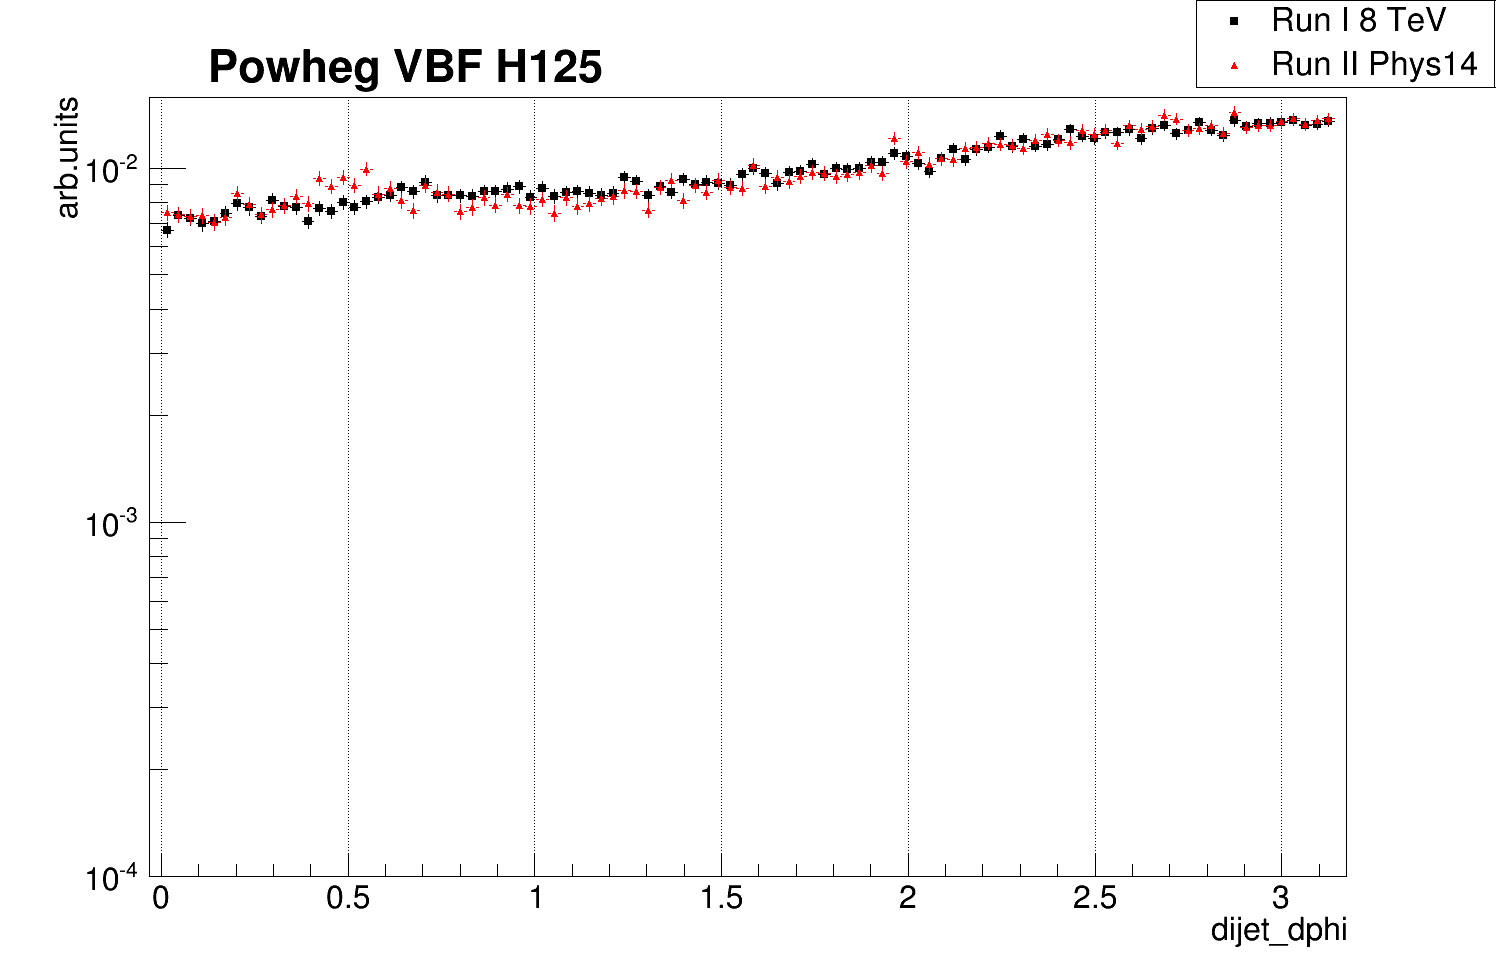
\includegraphics[width=.5\textwidth]{TalkPics/unskimmedsigmc060715/dijet_dphi_log.png}
  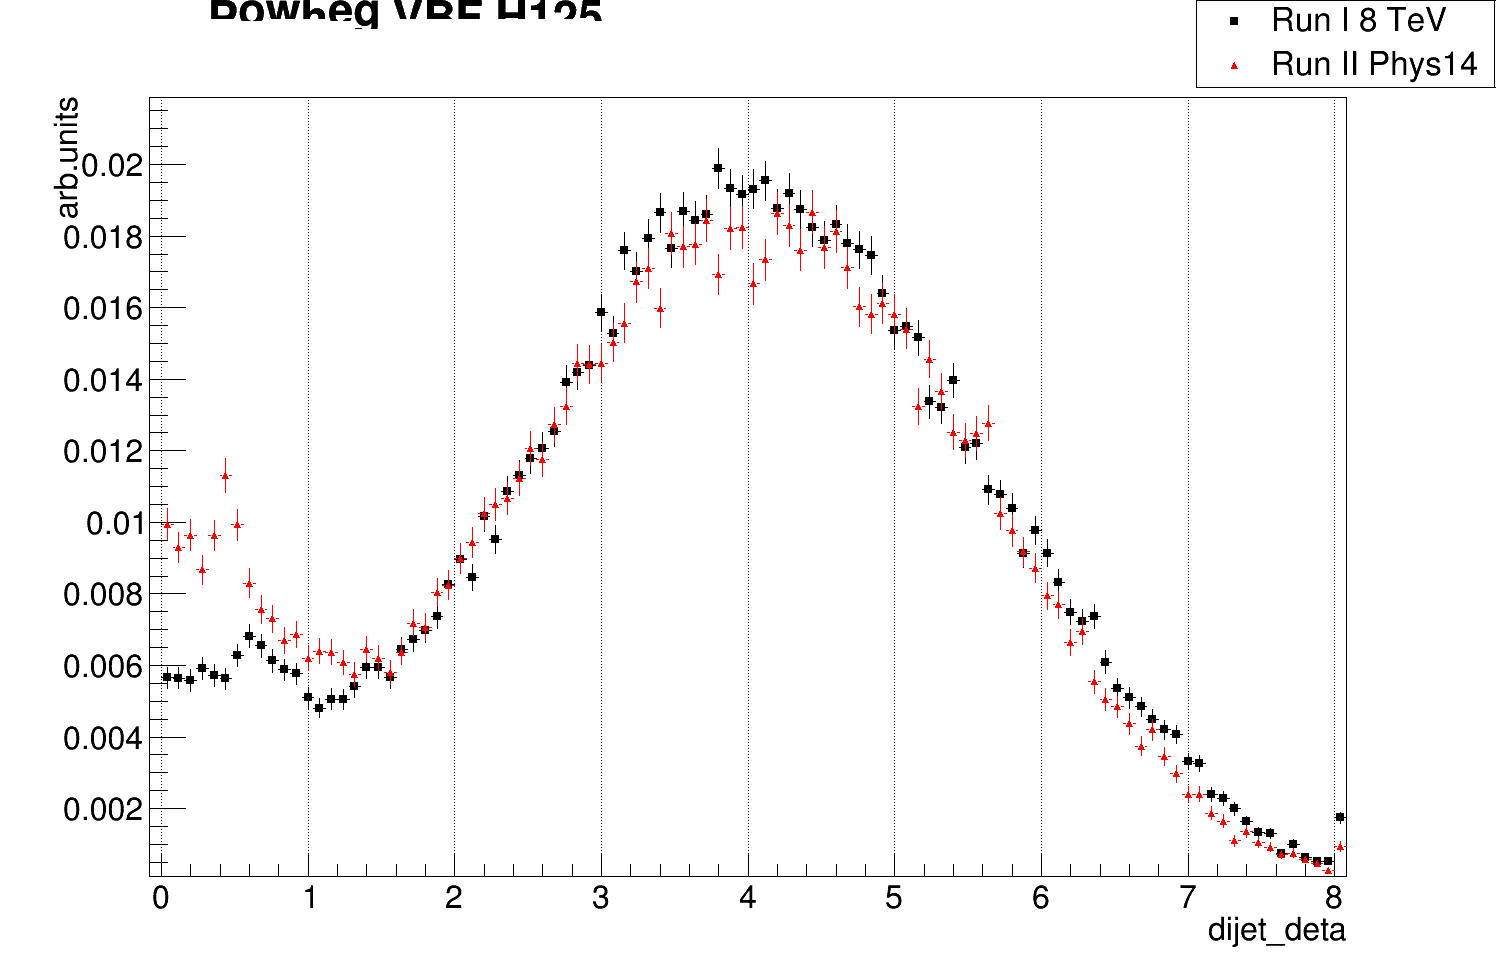
\includegraphics[width=.5\textwidth]{TalkPics/unskimmedsigmc060715/dijet_deta_nolog.png}
  
\end{frame}

\begin{frame}
  \begin{block}{Spring 15 samples}
    \begin{itemize}
    \item MiniAOD now available for $m_{H}=$ 110,300 GeV
    \item PU Jet ID can now be rerun if we want AK4PF jets
    \item[-] Decided yesterday to attempt to keep both AK4PF and AK4PFCHS and also possibly add PUPPI
    \item Also decided to add mvaMET to ntuples
    \item[-] Chayanit suggested this may become a MET POG recommendation
    \end{itemize}
  \end{block}
\end{frame}

\begin{frame}
  \label{lastframe}
  \begin{block}{Summary}
    \begin{itemize}
    \item Neutrinos included in gen jets for Phys14 samples
    \item[-] Usefulness of samples for gen studies is therefore limited
    \item Spring 15 samples are becoming available
    \item[-] We should move to these as soon as possible
    \end{itemize}
  \end{block}
\end{frame}

\begin{frame}
  \frametitle{Backup}
\end{frame}

\end{fmffile}
\end{document}
